Die hier besprochenen Grundlagen gehen nicht in eine Tiefe, um alle evtl. Fragen zu klären. Jedes einzelne Gebiet könnte eine Arbeit füllen. Stattdessen sollen lediglich einen kleinen Einblick geben.
\section{Künstliche Intelligenz}
Die Grafik \ref{img:classification_of_terms} soll die Einordnung von LLMs im Bereich der künstlichen Intelligenz zeigen.
\begin{figure}[!ht]
	\includegraphics[width=0.8\textwidth]{content/chapter_basics/images/einordnung_bezeichnungen.eps}
	\centering
	\caption{Einordnung LLMs}
	\label{img:classification_of_terms}
\end{figure}

In den folgenden Kapiteln werden die wichtigsten Technologien und Begriffe erläutert.\vspace{0.2cm}

Eine explizite Definition für künstliche Intelligenz ist zurzeit noch nicht erfolgt. Geschuldet ist diese Tatsache, da der Begriff Intelligenz nicht eindeutig definiert ist. Somit finden sich viele Versuche eine Definition für künstliche Intelligenz herzuleiten. In dieser Arbeit wird die Definition aus \cite[6 ff.]{definition_ki2019} verwendet.

\epigraph[text indent=0.5cm]{
	Systeme der künstlichen Intelligenz (KI-Systeme) sind vom Menschen entwickelte Softwaresysteme (und gegebenenfalls auch Hardwaresysteme)3, die in Bezug auf ein komplexes Ziel auf physischer oder digitaler Ebene handeln, indem sie ihre Umgebung durch Datenerfassung wahrnehmen, die gesammelten strukturierten oder unstrukturierten Daten interpretieren, Schlussfolgerungen daraus ziehen oder die aus diesen Daten abgeleiteten Informationen verarbeiten, und über das bestmögliche Handeln zur Erreichung des vorgegebenen Ziels entscheiden. KI-Systeme können entweder symbolische Regeln verwenden oder ein numerisches Modell erlernen, und sind auch in der Lage, die Auswirkungen ihrer früheren Handlungen auf die Umgebung zu analysieren und ihr Verhalten entsprechend anzupassen.
}

(\href{https://www.bitkom.org/sites/main/files/file/import/171012-KI-Gipfelpapier-online.pdf}{Wirtschaftliche Bedeutung ...}, 26 ff.).

\subsection{Historisches}
% aus: https://www.perplexity.ai/page/a-historical-overview-of-ai-wi-A8daV1D9Qr2STQ6tgLEOtg

An dieser Stelle eine kleine historische Exkursion in der Entwicklung der künstlichen Intelligenz.\vspace{0.2cm}

\begin{figure}[!ht]
	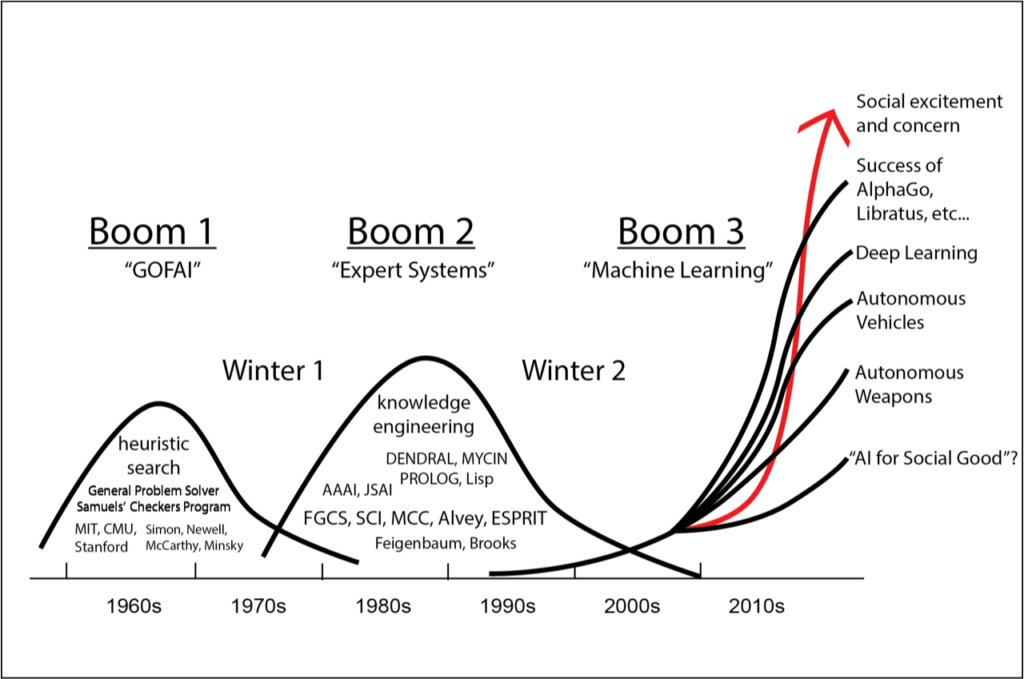
\includegraphics[width=0.8\textwidth]{content/chapter_basics/images/ai-winter-cycles.jpg}
	\centering
	\caption{KI Winterzyklen}
	\label{img:ai_winter_cycles}
\end{figure}

\textbf{1966: Rückschläge bei der maschinellen Übersetzung}\vspace{0.2cm}

\textbf{1969: Auswirkungen der Perzeptron-Kritik}\vspace{0.2cm}

\textbf{1971-75: Die Finanzierungsherausforderungen der DARPA}\vspace{0.2cm}

\textbf{1973: Der Fallout des Lighthill-Berichts}\vspace{0.2cm}

\textbf{1973-74: Kürzung der DARPA-Mittel}\vspace{0.2cm}

\textbf{1987: Zusammenbruch der LISP-Maschine}\vspace{0.2cm}

\textbf{1988: Kürzungen bei der strategischen Datenverarbeitung}\vspace{0.2cm}

\textbf{1990er Jahre: Niedergang von Expertensystemen}\vspace{0.2cm}

\textbf{1990er Jahre: Ende des Projekts der fünften Generation}\vspace{0.2cm}

\textbf{KI-Frühling des frühen 21. Jahrhunderts}\vspace{0.2cm}



\subsection{Maschinelles Lernen}
Das Gebiet um maschinelles Lernen (eng. Machine Learning) ist ein Teilgebiet der Künstlichen Intelligenz. Für das maschinelle Lernen wird in dieser Arbeit die allgemein gültige Definition nach Tom M. Mitchell verwendet.\vspace{0.2cm}

\epigraph[
author={Mitchell, Tom M},
source={Machine Learning},
translation={Ein Computerprogramm lernt aus Erfahrung E in Bezug auf eine Klasse von Aufgaben T und ein Leistungsmaß P, wenn sich seine Leistung bei Aufgaben in T, gemessen an P, mit der Erfahrung E verbessert.}
]{
	A computer programm is said to learn from experience E with respekt to some class of tasks T and performance measure P, if its performance at tasks in T, as measured by P, improves with experience E.
}

Bei dieser Definition ist,\\
\textbf{E} die \textbf{Erfahrung}, die Daten aus denen das System lernt,\\
\textbf{T} beschreibt die \textbf{Aufgabe}, die das System erledigen soll und\\
\textbf{P} ist die \textbf{Leistungskennzahl} an dem der Erfolg des Systems die Aufgabe zu lösen gemessen wird.\vspace{0.2cm}
%Da es mehrere Definitionen maschinellen Lernens gibt definieren WITTEN ET AL. (2001:6) eine operationale Definition von Lernen: „Etwas lernt, wenn es sein Verhalten so ändert, dass es in Zukunft eine bessere Leistung aufweist.“

Maschinelles Lernen (\acrshort{ML}) und Künstliche Intelligenz (\acrshort{KI}) sind nicht wirklich in der Lage selbstständig zu lernen oder denken, sie imitieren dies lediglich nach. Das maschinelle Lernen ist aber wohl in der Lage komplexe Muster und Funktionen in großen Datenmengen zu erkennen. Durch die Unfähigkeit zu lernen kann KI keine neuen Inhalte schaffen.\vspace{0.3cm}

Es ist auch egal wie gut die Modelle trainiert werden, eine 100\% Fehlerfreiheit gibt es nicht. Für die Praxis bedeutet dies, die Ausgaben von Modellen müssen durch Menschen immer wieder evaluiert werden, um dessen Richtigkeit sicherzustellen. Zudem sollten keine Modelle verwendet werden, wenn die Lösung eines Problems durch einen konkreten Algorithmus erfolgen kann. Hier können die Ergebnisse nachvollzogen werden und sind für den Menschen besser zu verstehen.\vspace{0.2cm}

\begin{figure}[!ht]
	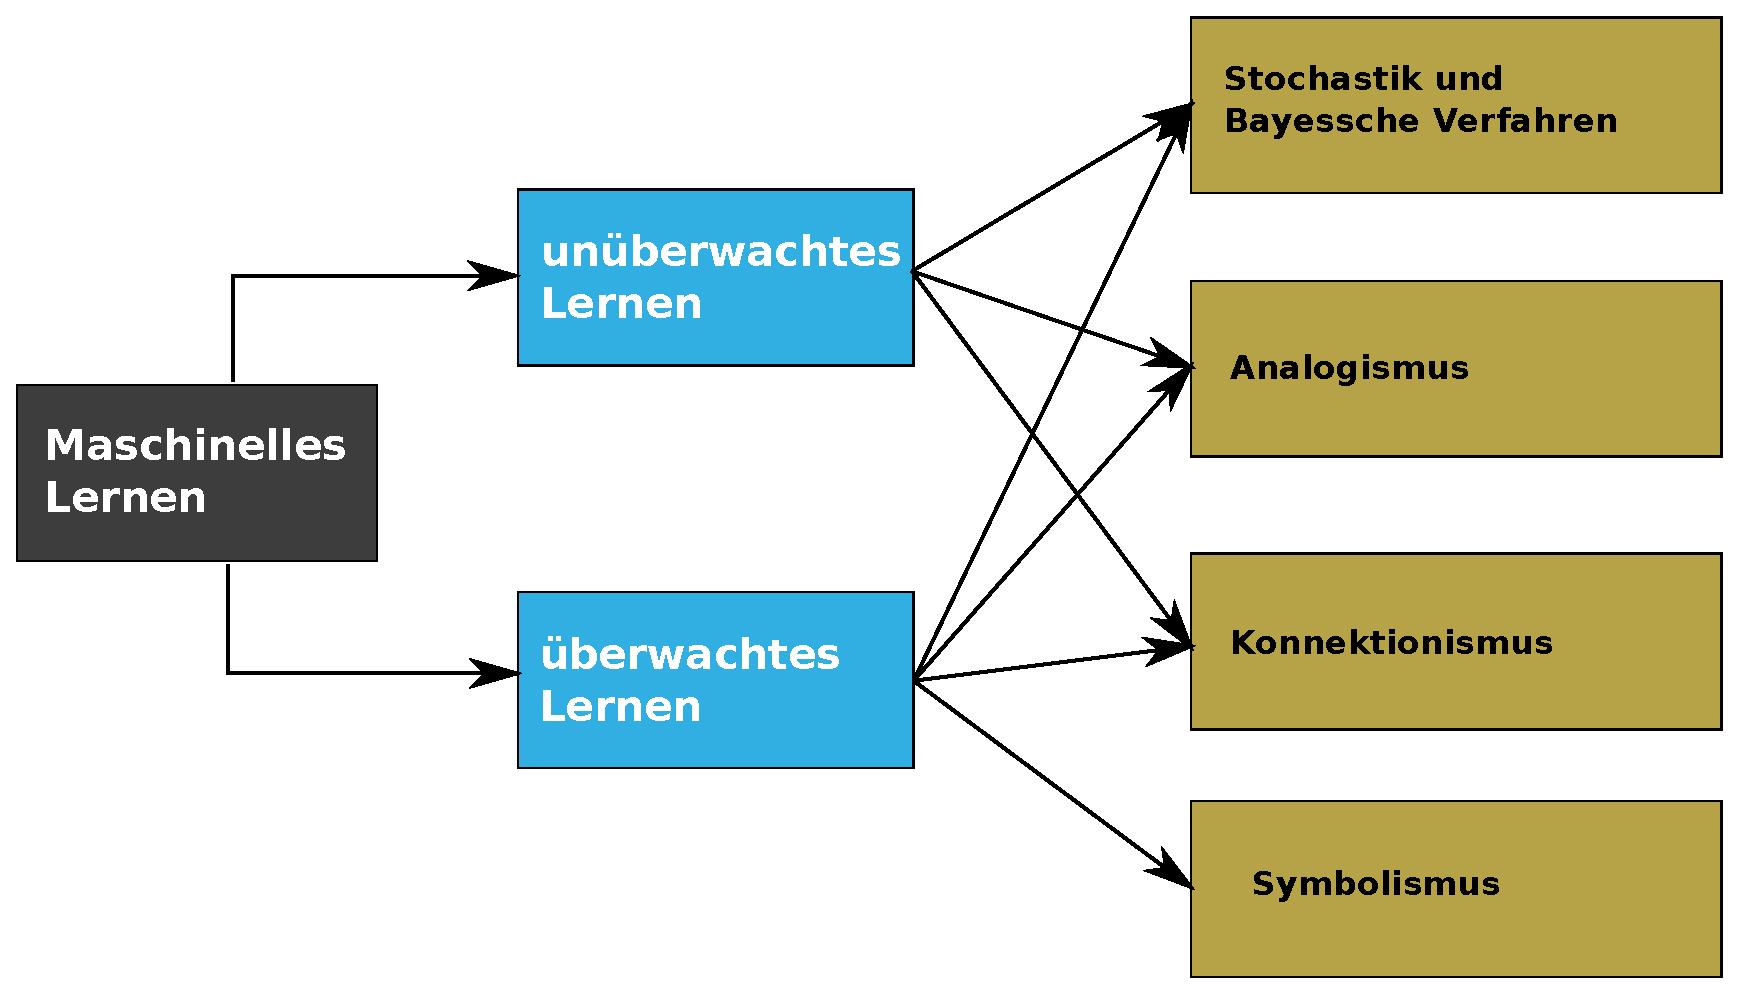
\includegraphics[width=0.8\textwidth]{content/chapter_basics/images/learning_paradigmen_ml_v2.eps}
	\centering
	\caption{Lernparadigmen des maschinellen Lernens}
	\label{img:learning_paradigms_of_ml}
\end{figure}


\subsection{Lernparadigmen des ML}
Das maschinelle Lernen wird in zwei wichtige Formen der Lernparadigmen unterteilt. Dem überwachten und dem unüberwachten Lernen. Abbildung \ref{img:learning_paradigms_of_ml} zeigt die wichtigsten Lernparadigmen des maschinellen Lernens.

\subsubsection{Überwachtes Lernen}
Bei überwachten Lernen sind für die Eingaben der Trainingsdaten dazugehörige Ausgaben (Labels) definiert. Das Ziel ist es eine Funktion zu trainieren um künftige Eingaben korrekt klassifizieren oder vorhersagen zu können.

\subsubsection{Unüberwachtes Lernen}
Bei unüberwachten Lernen sind die gelabelten Ausgaben nicht vorhanden. Hierbei wird beispielsweise durch Clustering oder Dimensionsreduktion versucht Muster und Strukturen zu erkennen.


\subsection{Theoretische Grundlagen}
In den folgenden Kapiteln werden vier wichtige Konzepte zum maschinellen Lernen besprochen. 

\subsubsection{Stochastik und Bayessche Verfahren}
Als Teilgebiet der Mathematik befasst sich die Stochastik mit Wahrscheinlichkeiten und zufälligen Prozessen. Auf dem Gebiet des maschinellen Lernens werden mithilfe der Stochastik Prognosen erstellt.\vspace{0.2cm}

Bei den Bayesschen Verfahren handelt es sich um stochastische Methoden, die auf dem Bayes-Theorem basieren. Hierbei werden neue Daten berücksichtigt, um die Wahrscheinlichkeit zu aktualisieren.\vspace{0.2cm}

Beide Methoden finden im überwachten und unüberwachtes Lernen Anwendung.

\subsubsection{Analogismus}
Dieser Lernansatz sucht nach Ähnlichkeiten in den Daten. Er basiert auf der Annahme, dass ähnliche Daten ähnliche Vorhersagen oder Klassifizierungen besitzen. Dieses Modell lernt, indem neue Daten mit bekannten vergleicht und nach ähnlichen Strukturen und Mustern sucht. Ein bekanntes Verfahren für diesen Lernansatz ist der k-Nearest Neighbors (\acrshort{k-NN}).\vspace{0.2cm}

Der Analogismus wird im überwachten Lernen als auch im unüberwachten Lernen angewandt, um Muster und Strukturen zuerkennen.

\subsubsection{Konnektionismus}
Der Lernansatz des Konnektionismus beruht auf kleine Einheiten die miteinander verbunden sind. Diese werden als Neuronen bezeichnet, die den Nervenzellen von Organismen nachempfunden sind. Die Künstlichen neuronalen Netze sind die bekanntesten Vertreter auf denen auch Deep Learning Modelle basieren.\vspace{0.2cm}

Auch dieser Lernansatz wird im unüberwachten und überwachten Lernen angewandt.

\subsubsection{Symbolismus}
Anders als beim Konnektionismus arbeiten die Einheiten beim Symbolismus mit explizite formale Regeln und Symbole, um das Wissen darzustellen. Der Symbolismus ist weniger flexible im Umgang mit unvollständigen Datensätzen und Unsicherheiten. Daher hat dieser Lernansatz weniger Relevanz als der Konnektionismus.\vspace{0.2cm}

Dieser Lernansatz findet im überwachten Lernen Anwendung, als Beispiel sind hier Entscheidungsbäume zu nennen.


\subsection{Neuronale Netze}
KNN

\subsubsection{Neuronen im neuronalen Netz}
Neuronen

\subsubsection{Arten der neuronalen Netzen}
KNN Arten

\subsubsection{Lernprozess im neuronalen Netz / Training}
Training

\subsection{Deep Learning}
DL

\subsection{Natural Language Processing}
NPL

\section{Large Language Model}
Large Language Model

\subsection{Grundlagen}
Grundlagen

\subsubsection{Tokenisierung}
Token

\subsubsection{Embedding}
Embedding

\subsubsection{Vorhersage}
Transformer

\subsubsection{Dekodierung}
Dekodierung

\subsection{Historie der LLM}
Historie

%\subsection{Weitere Begriffe bei LLMs}
%LLMs

%\subsubsection{Halluzinationen}

\section{Orchestrierung von LLMs}
Orchestrierung

\section{Multi-Agenten-Systeme}
Multi-Agent-System

\section{Prompt Engineering}
Prompt

\section{Grundlagen bei der Entwicklung von Webanwendungen}
Webanwendung
